\label{chapter:campusjobs} 
\section{Introduction}

Campus computing is usually defined as a cluster, or a set of clusters available to researchers for computational computing.  These clusters are divided either by purpose, i.e. owned by a certain group, or by hardware generations.  Users submit to a single cluster, and their jobs are eligible to run on that cluster.  We propose a framework to distribute jobs to multiple campus clusters transparently to the user.  We named our framework Bosco.  It provides:
\begin{itemize}
\item Easy and non-root installation.  No administrative intervention is required to install and start Bosco on either the submitter or the cluster.
\item Connections to the remote cluster using common, non-custom, protocols
\item Transparent load balancing across multiple clusters.
\end{itemize}

In this chapter I will discuss the methods developed to aid in distributed scientific computing on a research campus using Bosco.  

\section{Bosco Architecture}
\label{sec:boscoarch}

% Flow of job (from picture)
% Installer improvement
% 

The Bosco user experience can be described in 2 sections: installation/configuration and running jobs.  Each of these areas were approached with the goal of improving the typical user experience for installing and running distributed computing software.

The Bosco architecture is divided into the submit host and the cluster login node.  The submit host is where the user submits their jobs and where the user interacts with the Bosco system.  The login node is the submit host for a cluster.  The login node is assumed to not be maintained by the user submitting to Bosco.  The login node has access to the local scheduler with commands such as \texttt{qsub} and \texttt{qstat} (for PBS).  

\subsection{Installation \& Configuration}
Though typically separate, Bosco combined the installation and configuration steps in order to improve the user experience.  Both are done by a single script, the \texttt{bosco\_quickstart} script that follows several steps:

\begin{enumerate}
\item Determine the platform and download the appropriate version of Bosco (supports Mac, EL5/6, Debian 6)
\item Install Bosco into the user's home directory.
\item Prompt the user for details of connecting their first cluster to Bosco.
\end{enumerate}

The script downloads the Bosco binaries from a central server to the submit host.  Bosco is installed into the user's home directory by default in order to enable non-root installations.  Connecting a cluster to the Bosco submit host requires configuring the secure connection to the cluster, and installing a small amount of software on the submit node that will be used for job submission and job status checks.

We have also created a native installer, a PKG, for the Mac version of Bosco.  It is distributed in an Apple Disk Image (DMG) for consistency with other Mac software.  Unlike the Linux installer, It does not automatically configure a cluster at first installation.


\subsection{Running Jobs}

The image shown in Figure \ref{fig:archgraph1} shows the architecture of job submissions of a Bosco submit node.  Job submissions are done from the Bosco submit host, which in turn submit to the connected cluster login node.  

\begin{figure}[ht!]
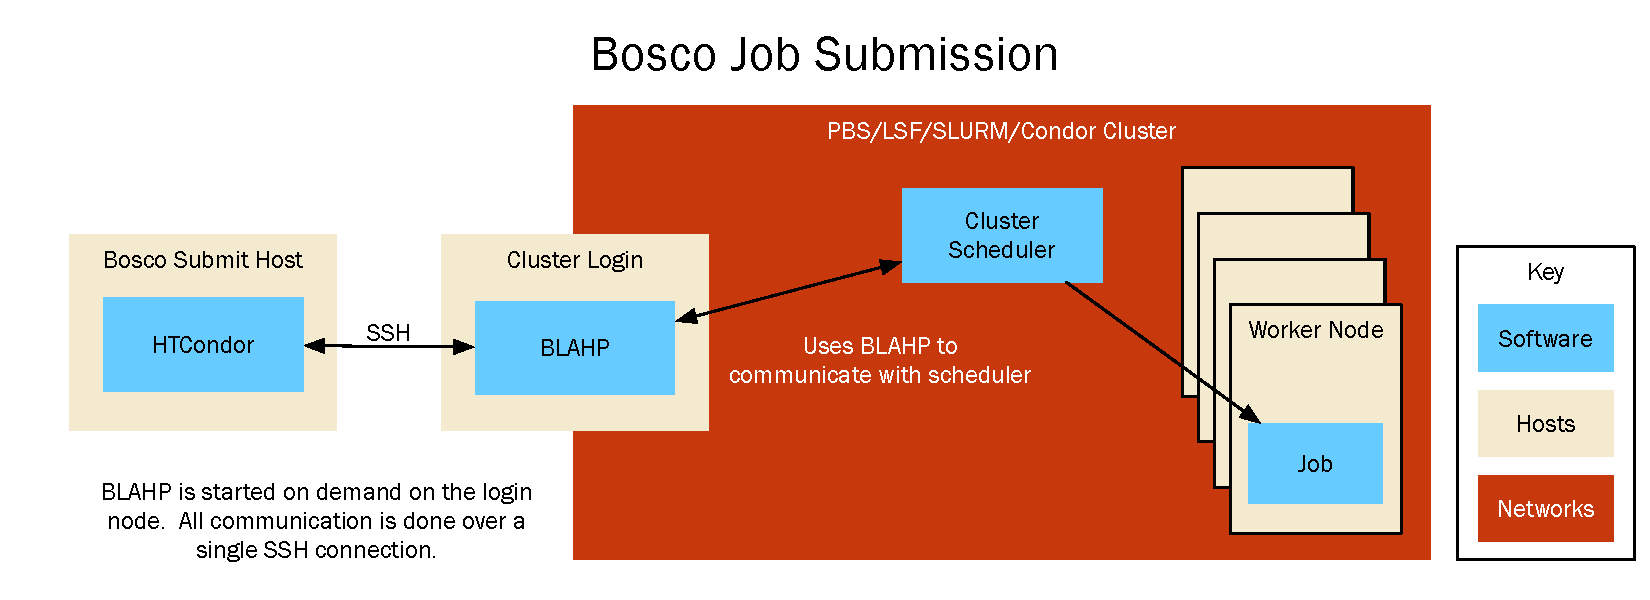
\includegraphics[width=\textwidth]{images/ArchitectureGraph1}
\caption{Bosco Architecture}
\label{fig:archgraph1}
\end{figure}

First, the Bosco submit node connects to the login node over an SSH connection and creates the forwarded SSH connection back to the submit node which is used for file transfer.  It creates the forwarded SSH connection in order to minimize the number of necessary connections between the Bosco submit host and the login node.  By reusing the same SSH connection, we reduce the number of necessary connections and SSH logins to 1.  Further, the number of connections is not dependent on the number of jobs, as Bosco will reuse the same connection for all jobs submitted to a cluster.  Minimizing the number of connections to a login node is important since many login nodes include firewall rules to slow down brute force SSH logins that block frequent successive SSH connections.  The Bosco submit host does not require any open ports in a firewall, only outgoing connections to remote login node's SSH port.

Next, Bosco checks for the necessary installed software on the login node, and starts the BLAHP \cite{blahp} daemon that will communicate with the scheduler on the login node.  The BLAHP daemon on the login node starts the file transfer daemon to connect back to the submit host through a forwarded SSH tunnel that Bosco created.  The transfer daemon creates and transfers the job sandbox to the login node.  The transfer to the login node is performed by HTCondor's fault tolerant file transfer mechanisms and are entirely encrypted over the SSH connection.  Authentication between the login node and the Bosco submit host is performed by a shared secret that was previously sent over the SSH connection to the BLAHP daemon.

After the files have been transferred, Bosco sends the job's submission ClassAd \cite{raman1998matchmaking} to the BLAHP daemon to translate to the local site's scheduler language.  The BLAHP supports PBS \cite{computing2013torque}, LSF \cite{computinglsf}, SGE \cite{gentzsch2001sun}, SLURM \cite{yoo2003slurm}, and HTCondor schedulers.  The BLAHP creates the submission file, and submits to the cluster's scheduler.  Bosco periodically polls the BLAHP over the SSH connection for the status of the job.  Once the job is detected to have been completed, the BLAHP starts HTCondor's transfer daemon to transfer the output sandbox back to the submitter machine.

\subsection{Improving User Experience}

In order to improve the user experience, at each step of the job process extra effort has been given to provide useful error messages in case of failures.  For example, HTCondor was modified to relay the standard error for any commands sent to the BLAHP daemon, as useful debugging information is available there.  

Also, an additional \emph{traceroute} was created to test each step of the job submission process, including:

\begin{enumerate}
\item SSH connection to the remote login host.  Tests network connection, login host availability, passwordless SSH setup.
\item Job submission to the Bosco submit host.  Tests Bosco daemon availability, Bosco submit host file system availability.
\item Job submission to the remote login host.  Tests the remote scheduler availability, remote cluster software setup, input file transfer, cluster file system availability.
\item Job completion and status update from login host.  Tests Bosco status check process, output file transfer.
\end{enumerate}

The \emph{traceroute} is very useful for debugging issues with a Bosco installation.  It is designed to test each step in the job execution life cycle and give meaningful error messages and possible solutions.

\section{Load Balanced Access to Computational Resources}

Bosco is used in conjunction with the Campus Factory \cite{website:campusfactory}, which is described in full in my Master's thesis \cite{weitzel2011campus}.  The Campus factory submits pilot jobs to remote clusters to create an overlay that provides a consistent interface to the resources.  The campus factory submits to multiple Bosco endpoints simultaneously, load balancing between them by keeping idle jobs (constant pressure) on all clusters.

Submission via the Bosco framework is done using the HTCondor submit syntax.  When an idle user job is detected by the Campus Factory, it begins to submit glide ins to all Bosco endpoints simultaneously.  The Campus Factory maintains idle glideins on each of the endpoints until the user jobs have completed.  The jobs run on any resources that become available.


\section{Conclusion}

Bosco and the Campus Factory combine to make an easy to use framework that can distribute jobs to many computational clusters on a campus.  Users are able to effectively distribute their processing to multiple clusters using this framework.  In my dissertation, I will show that Bosco transparently and effectively distributes computational jobs across multiple clusters on a campus, while maintaining simple usage for users.

I will measure the efficiency of the load distribution across multiple resources.  When the jobs are sent across multiple resources, the expected result is a decreased time to completion due to multiple available resources.  But, the framework that allows for load balancing can cause increased overhead due to multiple levels of scheduling, first at the local cluster scheduler, then at the user's Bosco submit host.

If the user's workflow requires significant data, it may be inefficient to use Bosco's transfer mechanisms which are bottlenecked by the transfer speed of the Bosco submit host.  This will be another metric against which to measure Bosco's effectiveness.  It is expected that large datasets will not be an efficient use of Bosco.  Therefore, we will introduce a policy language in Chapter \ref{chapter:campusdata} that will allow the user to express preferred transfer methods, and finally another transfer method that can be utilized with Bosco in Chapter \ref{chapter:coordinatingstorage}.



